%% Oct 2004; edited by OR
%%version Feb 3, 2001; last edited by SA
\documentclass[11pt]{article}
%\usepackage{lucidbry}
%\usepackage{trees}
\usepackage{mathtools}
\usepackage[sc]{mathpazo}
%\usepackage{txfonts}
\linespread{1.05}         % Palatino needs more leading (space between lines)
\usepackage[T1]{fontenc}

\usepackage{amsmath}
\usepackage{amssymb}
%\usepackage{mnsymbol}
%\usepackage{mathabx}
%\usepackage{fdsymbol}

%\usepackage{accents}
%\usepackage{times}
\usepackage{ntheorem}
\usepackage{latexsym}
\usepackage{xspace}
\usepackage{fancyhdr}
%\usepackage{psfig}
%\usepackage{epsfig}
\usepackage{graphicx}
\usepackage{epspdfconversion}
%\DeclareGraphicsExtensions{.pdf,.eps,.png,.jpg}
\usepackage{hyperref}
\usepackage[ruled]{algorithm2e}
\newcommand\mycommfont[1]{\rmfamily{\it #1}}
\SetCommentSty{mycommfont}

\usepackage{float}
\usepackage{subfigure}
\usepackage{color}
%\usepackage{lucmath}

%tTHEOREM TYPE ENVIRONMENTS
%\theoremstyle{break}
\theoremheaderfont{\scshape}
\theorembodyfont{\slshape}
\newtheorem{theorem}{Theorem}
\newtheorem{corollary}[theorem]{Corollary}
\newtheorem{lemma}[theorem]{Lemma}
\newtheorem{proposition}[theorem]{Proposition}
\theoremstyle{plain}
\theorembodyfont{\rmfamily}
\newtheorem{problem}{Problem}
\newtheorem{observation}[theorem]{Observation}
\newtheorem{remark}[theorem]{Remark}
\theorembodyfont{\itshape}
\newtheorem{fact}[theorem]{Fact}
\newtheorem{definition}[theorem]{Definition}
\newtheorem{assumption}[theorem]{Assumption}
\newtheorem{claim}[theorem]{Claim}
\newenvironment{proof}{\noindent {\sc Proof:}}{$\Box$ \medskip}
\newenvironment{proofof}[1]{\noindent {\sc Proof of #1:}}{$\Box$ \medskip}
\theoremstyle{plain}
\theorembodyfont{\normalfont}
\theoremheaderfont{\normalfont\bfseries}
\newtheorem{exercise}{Exercise}

% {\renewcommand{\labelenumi}{\S\theenumi}
%    \begin{enumerate}}{\end{enumerate}}


% \setlength{\oddsidemargin}{.25in}
% \setlength{\evensidemargin}{.25in}
% \setlength{\textwidth}{6in}
% \setlength{\topmargin}{-0.4in}
% \setlength{\textheight}{8.5in}

\usepackage{fullpage}

% Jan 2013, edited by DD
% Oct 2004, edited by OR
%%Version Feb 3 2001; last edited by SA
% Feb 13, 2001: LT adds following macros:
%  \logred, \conl, \genclass, \cogenclass, \size,
%  \floor, \ceil, \comp, \ffigure, \ffigureh
%  \iff, \implies, \sigmatwo, \sigmathree, \pitwo,
%  \scand, \scor, \scnot, \scyes
%Feb20 SA added \sig and \pip for boldface polynomial hierarchy
%% Macros for complexity theory notation
%% Complexity classes



%% Notation for integers, natural numbers, reals, fractions, sets, cardinalities
%%and so on

\newcommand\B{\{0,1\}}      % boolean alphabet  use in math mode
\newcommand\Bs{\{0,1\}^*}   % B star            use in math mode
\newcommand\true{\mbox{\sc True}}
\newcommand\false{\mbox{\sc False}}
\DeclareRobustCommand{\fracp}[2]{{#1 \overwithdelims()#2}}
\DeclareRobustCommand{\fracb}[2]{{#1 \overwithdelims[]#2}}
\newcommand{\marginlabel}[1]%
{\mbox{}\marginpar{\it{\raggedleft\hspace{0pt}#1}}}
\newcommand\card[1]{\left| #1 \right|} %cardinality of set S; usage \card{S}
\newcommand{\comp}[1]{\overline{#1}}
\newcommand{\tran}[1]{{#1}^T}


%% Various things to write in small caps
\def\scand{\mbox{\sc and}}
\def\scor{\mbox{\sc or}}
\def\scnot{\mbox{\sc not}}
\def\scyes{\mbox{\sc yes}}
\def\scno{\mbox{\sc no}}
\def\scmaybe{\mbox{\sc maybe}}

% new epsilons
\newcommand{\eps}{\varepsilon}
\renewcommand{\epsilon}{\varepsilon}

\def\lecturegg{7}

% GENERAL COMPUTING STUFF
\newcommand{\bit}{\ensuremath{\set{0,1}}}
\newcommand{\pmone}{\ensuremath{\set{-1,1}}}

% asymptotic stuff
\DeclareMathOperator{\poly}{poly}
\DeclareMathOperator{\polylog}{polylog}
\DeclareMathOperator{\negl}{negl}
\newcommand{\Otil}{\ensuremath{\tilde{O}}}

% probability/distribution stuff
\DeclareMathOperator*{\E}{\mathbb{E}}
\DeclareMathOperator*{\Var}{Var}

% assorted
\DeclareMathOperator*{\wt}{wt}

% hash functions
\newcommand{\calH}{\ensuremath{\mathcal{H}}}
\newcommand{\calX}{\ensuremath{\mathcal{X}}}
\newcommand{\calY}{\ensuremath{\mathcal{Y}}}
\newcommand{\calL}{\ensuremath{\mathcal{L}}}
\newcommand{\calB}{\ensuremath{\mathcal{B}}}

\newcommand{\compind}{\ensuremath{\stackrel{c}{\approx}}}
\newcommand{\statind}{\ensuremath{\stackrel{s}{\approx}}}
\newcommand{\perfind}{\ensuremath{\equiv}}

% font for general-purpose algorithms
\newcommand{\algo}[1]{\ensuremath{\mathsf{#1}}}

% font for complexity classes
\newcommand{\class}[1]{\ensuremath{\mathsf{#1}}}

% complexity classes and languages
\renewcommand{\P}{\class{P}}
\newcommand{\BPP}{\class{BPP}}
\newcommand{\NP}{\class{NP}}
\newcommand\RP{\class{RP}}
\newcommand\ZPP{\class{ZPP}}
\newcommand{\coNP}{\class{coNP}}
\newcommand{\AM}{\class{AM}}
\newcommand{\coAM}{\class{coAM}}
\newcommand{\IP}{\class{IP}}
\newcommand{\SZK}{\class{SZK}}
\newcommand{\NISZK}{\class{NISZK}}
\newcommand{\NICZK}{\class{NICZK}}
\newcommand{\PPP}{\class{PPP}}
\newcommand{\PPAD}{\class{PPAD}}

% \newcommand\SIGMA2{\class{$\Sigma_2$}}
% \newcommand\SIGMA3{\class{$\Sigma_3$}}
% \newcommand\PI2{\mbox{\bf $\Pi_2$}\xspace}
\newcommand\PH{\mbox{\bf PH}\xspace}
\newcommand\PSPACE{\mbox{\bf PSPACE}\xspace}
\newcommand\NPSPACE{\mbox{\bf NPSPACE}\xspace}
\newcommand\DL{\mbox{\bf L}\xspace}
\newcommand\NL{\mbox{\bf NL}\xspace}
\newcommand\coNL{\mbox{\bf coNL}\xspace}
\newcommand\sharpP{\mbox{\#{\bf P}}\xspace}
\newcommand\parityP{\mbox{$\oplus$ {\bf P}}\xspace}
\newcommand\PCP{\mbox{\bf PCP}}
\newcommand\DTIME{\mbox{\bf DTIME}}
\newcommand\NTIME{\mbox{\bf NTIME}}
\newcommand\DSPACE{\mbox{\bf SPACE}\xspace}
\newcommand\NSPACE{\mbox{\bf NSPACE}\xspace}
\newcommand\CNSPACE{\mbox{\bf coNSPACE}\xspace}
\newcommand\EXPTIME{\mbox{\bf EXPTIME}\xspace}
\newcommand\NEXPTIME{\mbox{\bf NEXPTIME}\xspace}
\newcommand\GENCLASS{\mbox{$\cal C$}\xspace}
\newcommand\coGENCLASS{\mbox{\bf co$\cal C$}\xspace}
\newcommand\SIZE{\mbox{\bf SIZE}\xspace}
\newcommand\sig{\mathbf \Sigma}
\newcommand\pip{\mathbf \Pi}

%%Computational problems
\newcommand\sat{\mbox{SAT}\xspace}
\newcommand\tsat{\mbox{3SAT}\xspace}
\newcommand\tqbf{\mbox{TQBF}\xspace}


\newcommand{\yes}{\ensuremath{\text{YES}}}
\newcommand{\no}{\ensuremath{\text{NO}}}

\newcommand{\Piyes}{\ensuremath{\Pi^{\yes}}}
\newcommand{\Pino}{\ensuremath{\Pi^{\no}}}

% macros for matrices and vectors
\newcommand{\matA}{\ensuremath{\mathbf{A}}}
\newcommand{\matB}{\ensuremath{\mathbf{B}}}
\newcommand{\matC}{\ensuremath{\mathbf{C}}}
\newcommand{\matD}{\ensuremath{\mathbf{D}}}
\newcommand{\matE}{\ensuremath{\mathbf{E}}}
\newcommand{\matF}{\ensuremath{\mathbf{F}}}
\newcommand{\matG}{\ensuremath{\mathbf{G}}}
\newcommand{\matH}{\ensuremath{\mathbf{H}}}
\newcommand{\matI}{\ensuremath{\mathbf{I}}}
\newcommand{\matJ}{\ensuremath{\mathbf{J}}}
\newcommand{\matK}{\ensuremath{\mathbf{K}}}
\newcommand{\matL}{\ensuremath{\mathbf{L}}}
\newcommand{\matM}{\ensuremath{\mathbf{M}}}
\newcommand{\matN}{\ensuremath{\mathbf{N}}}
\newcommand{\matO}{\ensuremath{\mathbf{O}}}
\newcommand{\matP}{\ensuremath{\mathbf{P}}}
\newcommand{\matQ}{\ensuremath{\mathbf{Q}}}
\newcommand{\matR}{\ensuremath{\mathbf{R}}}
\newcommand{\matS}{\ensuremath{\mathbf{S}}}
\newcommand{\matT}{\ensuremath{\mathbf{T}}}
\newcommand{\matU}{\ensuremath{\mathbf{U}}}
\newcommand{\matV}{\ensuremath{\mathbf{V}}}
\newcommand{\matW}{\ensuremath{\mathbf{W}}}
\newcommand{\matX}{\ensuremath{\mathbf{X}}}
\newcommand{\matY}{\ensuremath{\mathbf{Y}}}
\newcommand{\matZ}{\ensuremath{\mathbf{Z}}}
\newcommand{\matzero}{\ensuremath{\mathbf{0}}}

\newcommand{\veca}{\ensuremath{\mathbf{a}}}
\newcommand{\vecb}{\ensuremath{\mathbf{b}}}
\newcommand{\vecc}{\ensuremath{\mathbf{c}}}
\newcommand{\vecd}{\ensuremath{\mathbf{d}}}
\newcommand{\vece}{\ensuremath{\mathbf{e}}}
\newcommand{\vecf}{\ensuremath{\mathbf{f}}}
\newcommand{\vecg}{\ensuremath{\mathbf{g}}}
\newcommand{\vech}{\ensuremath{\mathbf{h}}}
\newcommand{\veck}{\ensuremath{\mathbf{k}}}
\newcommand{\vecm}{\ensuremath{\mathbf{m}}}
\newcommand{\vecp}{\ensuremath{\mathbf{p}}}
\newcommand{\vecq}{\ensuremath{\mathbf{q}}}
\newcommand{\vecr}{\ensuremath{\mathbf{r}}}
\newcommand{\vecs}{\ensuremath{\mathbf{s}}}
\newcommand{\vect}{\ensuremath{\mathbf{t}}}
\newcommand{\vecu}{\ensuremath{\mathbf{u}}}
\newcommand{\vecv}{\ensuremath{\mathbf{v}}}
\newcommand{\vecw}{\ensuremath{\mathbf{w}}}
\newcommand{\vecx}{\ensuremath{\mathbf{x}}}
\newcommand{\vecy}{\ensuremath{\mathbf{y}}}
\newcommand{\vecz}{\ensuremath{\mathbf{z}}}
\newcommand{\veczero}{\ensuremath{\mathbf{0}}}

\renewcommand{\vec}[1]{\ensuremath{\mathbf{#1}}}

\DeclareMathOperator{\diag}{diag}

% blackboard symbols

\newcommand{\C}{\ensuremath{\mathbb{C}}}
\newcommand{\D}{\ensuremath{\mathbb{D}}}
\newcommand{\F}{\ensuremath{\mathbb{F}}}
\newcommand{\G}{\ensuremath{\mathbb{G}}}
\newcommand{\J}{\ensuremath{\mathbb{J}}}
\newcommand{\N}{\ensuremath{\mathbb{N}}}
\newcommand{\Q}{\ensuremath{\mathbb{Q}}}
\newcommand{\R}{\ensuremath{\mathbb{R}}}
\newcommand{\Z}{\ensuremath{\mathbb{Z}}}

\newcommand{\Zt}{\ensuremath{\Z_t}}
\newcommand{\Zp}{\ensuremath{\Z_p}}
\newcommand{\Zq}{\ensuremath{\Z_q}}
\newcommand{\ZN}{\ensuremath{\Z_N}}
\newcommand{\Zps}{\ensuremath{\Z_p^*}}
\newcommand{\ZNs}{\ensuremath{\Z_N^*}}
\newcommand{\JN}{\ensuremath{\J_N}}
\newcommand{\QRN}{\ensuremath{\mathbb{QR}_N}}

% Euclidean Ball
\newcommand{\ball}{\mathcal{B}_2}

% "left-right" pairs of symbols

% inner product
\newcommand{\pr}[2]{\langle{#1, #2}\rangle}
\newcommand{\prfit}[2]{\left\langle{#1, #2}\right\rangle}

% absolute value
\newcommand{\absfit}[1]{\left\lvert{#1}\right\rvert}
% a set
\newcommand{\set}[1]{\{{#1}\}}
\newcommand{\setfit}[1]{\left\{{#1}\right\}}
% parens
\newcommand{\parens}[1]{({#1})}
\newcommand{\parensfit}[1]{\left({#1}\right)}
% tuple, alias for parens
\newcommand{\tuple}[1]{\parens{#1}}
\newcommand{\tuplefit}[1]{\parensfit{#1}}
% square brackets
\newcommand{\bracks}[1]{[{#1}]}
\newcommand{\bracksfit}[1]{\left[{#1}\right]}
% rounding off
\newcommand{\round}[1]{\lfloor{#1}\rceil}
\newcommand{\roundfit}[1]{\left\lfloor{#1}\right\rceil}
% floor function
\newcommand{\floor}[1]{\lfloor{#1}\rfloor}
\newcommand{\floorfit}[1]{\left\lfloor{#1}\right\rfloor}
% ceiling function
\newcommand{\ceil}[1]{\lceil{#1}\rceil}
\newcommand{\ceilfit}[1]{\left\lceil{#1}\right\rceil}
% length of some vector, element
\newcommand{\length}[1]{\lVert{#1}\rVert}
\newcommand{\lengthfit}[1]{\left\lVert{#1}\right\rVert}
\newcommand{\eqdef}{\mathbin{\stackrel{\rm def}{=}}}

%transpose
\newcommand{\T}{\mathsf{T}}

% gram schmidt and dual bases
\newif\ifleo\leotrue
%\newif\ifleo\leofalse

\ifleo

\newcommand{\gs}[1]{{\vec #1}^\star}
\newcommand{\du}[1]{{\vec #1}^{\vee}}
\newcommand{\dl}[1]{{#1}^{\vee}}
\newcommand{\dgs}[1]{{\vec #1}^{\star}}
\newcommand{\mat}[1]{\vec{#1}}
\newcommand{\gsm}[1]{{\mat{#1}}^\star}
\newcommand{\dm}[1]{\mat{#1}^{\vee}}
\newcommand{\rdm}[1]{\mat{#1}^{\wedge}}%Reverse Dual
\newcommand{\dmt}[1]{\mat{#1}^{\vee \T}}
\newcommand{\dgsm}[1]{\mat{#1}^{*\vee}}

\else

\newcommand{\gs}[1]{\widetilde{\mathbf #1}}
\newcommand{\rgs}[1]{\accentset{\curvearrowleft}{\mathbf #1}}
\newcommand{\du}[1]{{\mathbf #1}^{*}}
\newcommand{\dl}[1]{{#1}^{*}}
\newcommand{\dgs}[1]{\widetilde{\mathbf #1}^{*}}
\newcommand{\rdgs}[1]{\accentset{\curvearrowleft}{\mathbf #1}^{*}}
\newcommand{\mat}[1]{\vec{#1}}
\newcommand{\gsm}[1]{\widetilde{\mat{#1}}}
\newcommand{\dm}[1]{\mat{#1}^*}
\newcommand{\rdm}[1]{{}^*\mat{#1}}%Reverse Dual
\newcommand{\dmt}[1]{\mat{#1}^{*\T}}
\newcommand{\dgsm}[1]{\widetilde{\mat{#1}}^{*}}

\fi

\newcommand{\vc}[1]{\vec{#1}}
\newcommand{\mt}[1]{\mat{#1}}

%\DeclareMathOperator*{\supp}{supp}
\DeclareMathOperator*{\conv}{conv}
\def\sym{\bigtriangleup}
\DeclareMathOperator*{\TVD}{d_{TV}}
\DeclareMathOperator*{\width}{width}
\DeclareMathOperator*{\argmax}{arg\,max}
\DeclareMathOperator*{\argmin}{arg\,min}
\DeclareMathOperator*{\cov}{cov}
\DeclareMathOperator{\SVP}{SVP}
\DeclareMathOperator{\HermiteSVP}{HermiteSVP}
\DeclareMathOperator{\CVP}{CVP}

%%% new commands -- norms, operators, blah blah.
\DeclarePairedDelimiter\norm{\lVert}{\rVert}
\DeclarePairedDelimiter\abs{\lvert}{\rvert}%
\newcommand{\enc}[1]{\langle #1 \rangle}
\makeatletter
\def\imod#1{\allowbreak\mkern10mu({\operator@font mod}\,\,#1)}
\makeatother

%%%% some other macros that can be cleaned up
\newcommand{\parl}[1]{\mathcal{P}(#1)}
\def\diag{\mathrm{diag}}
\def\Id{\mathrm{Id}}
\def\sph{\mathbb{S}}
\def\suchthat{\;:\;}
\def\psd{\succcurlyeq}
\def\minuszero{\setminus \set{\vec 0}}
\def\diam{\mathrm{Diam}}
\def\core{\mathcal{C}}
\def\st{~\mathrm{s.t.}~}
\def\linsp{\mathrm{span}}
\def\Gram{\mathrm{Gram}}
\def\vol{\mathrm{vol}}
\def\det{\mathrm{det}}
\def\supp{\mathrm{support}}
\def\lat{\mathcal{L}}
\def\aff{{\rm aff}}
\def\ext{{\rm ext}}
\def\cone{{\rm cone}}
\def\bd{{\rm bd}}
\def\relbd{{\rm relbd}}
\def\ker{{\rm ker}}
\def\d{{\rm d}}

\DeclareMathOperator*{\unif}{uniform}

%\newcommand\to{\rightarrow}
\newcommand{\from}{:}
\newcommand\xor{\oplus}
\newcommand\bigxor{\bigoplus}
\newcommand{\logred}{\leq_{\log}}
\def\iff{\Leftrightarrow}
\def\implies{\Rightarrow}

%% macros to write pseudo-code
\floatstyle{ruled}
\newfloat{procedure}{h!}{loa}
\floatname{procedure}{Procedure}

\newif\ifnewprog\newprogfalse

\ifnewprog

\newlength{\pgmtab}  %  \pgmtab is the width of each tab in the
\setlength{\pgmtab}{1em}  %  program environment
 \newenvironment{program}{\renewcommand{\baselinestretch}{1}%
\begin{tabbing}\hspace{0em}\=\hspace{0em}\=%
\hspace{\pgmtab}\=\hspace{\pgmtab}\=\hspace{\pgmtab}\=\hspace{\pgmtab}\=%
\hspace{\pgmtab}\=\hspace{\pgmtab}\=\hspace{\pgmtab}\=\hspace{\pgmtab}\=%
\+\+\kill}{\end{tabbing}\renewcommand{\baselinestretch}{\intl}}
\newcommand {\BEGIN}{{\bf begin\ }}
\newcommand {\ELSE}{{\bf else\ }}
\newcommand {\IF}{{\bf if\ }}
\newcommand {\FOR}{{\bf for\ }}
\newcommand {\TO}{{\bf to\ }}
\newcommand {\DO}{{\bf do\ }}
\newcommand {\WHILE}{{\bf while\ }}
\newcommand {\ACCEPT}{{\bf accept}}
\newcommand {\REJECT}{\mbox{\bf reject}}
\newcommand {\THEN}{\mbox{\bf then\ }}
\newcommand {\END}{{\bf end}}
\newcommand {\RETURN}{\mbox{\bf return\ }}
\newcommand {\HALT}{\mbox{\bf halt}}
\newcommand {\REPEAT}{\mbox{\bf repeat\ }}
\newcommand {\UNTIL}{\mbox{\bf until\ }}
\newcommand {\TRUE}{\mbox{\bf true\ }}
\newcommand {\FALSE}{\mbox{\bf false\ }}
\newcommand {\FORALL}{\mbox{\bf for all\ }}
\newcommand {\DOWNTO}{\mbox{\bf down to\ }}

\fi

%homework stuff
\definecolor{hintgray}{gray}{0.40}

%formatting commands
\newcounter{lecnum}
\newcommand{\lecture}[3]{%
%\pagestyle{myheadings}%
%\thispagestyle{plain}%
\newpage %
\setcounter{lecnum}{#1}%
\setcounter{page}{1}%
%\rule{\linewidth}{1mm}

 \thispagestyle{fancy}
 \headheight 45pt
 \lhead{\bf{Leiden, Spring 2024 \\ Lattices and their Algorithms} \vspace{.5em}\\ \hspace{1em}}
 \chead{{\Large \bf Lecture #1} \vspace{.5em} \\ \hrule height .5mm \hfill \\ {\bf \Large #2}}
 \rhead{\bf{Lecturers: L. Ducas \\ T.A.: #3} \vspace{.5em} \\ \hspace{1em}}
 \renewcommand{\headrulewidth}{1.2pt}
 \hspace{1em} \vspace{6pt}
}

\newcommand{\exercisedesc}[2]{%
 \newpage %
 \setcounter{lecnum}{#1}%
 \setcounter{page}{1}%

 \pagestyle{fancy}
 \headheight 30pt
 \lhead{\bf{Spring 2024 \\ Lattices and their Algorithms}}
 \chead{\bf{\large{Exercise #1 \\ Discussion on #2}}}
 \rhead{\bf{L. Ducas \\ Leiden}}
 \renewcommand{\headrulewidth}{1.2pt}
 \setlength{\headsep}{10pt}
}

\newcommand{\homeworkdesc}[2]{%
 \newpage %
 \setcounter{lecnum}{#1}%
 \setcounter{page}{1}%

 \pagestyle{fancy}
 \headheight 30pt
 \lhead{\bf{Spring 2024 \\Lattices and their Algorithms}}
 \chead{\bf{\large{Homework #1 \\ Due #2}}}
 \rhead{\bf{L. Ducas \\ Leiden}}
 \renewcommand{\headrulewidth}{1.2pt}
 \setlength{\headsep}{10pt}
}

\newcommand{\homeworksol}[1]{%
 \newpage %
 \setcounter{lecnum}{#1}%
 \setcounter{page}{1}%

 \pagestyle{fancy}
 \headheight 30pt
 \lhead{\bf{Spring 2024 \\ Lattices and their Algorithms}}
 \chead{\bf{\large{Partial Solutions to \\ Homework #1}}}
 \rhead{\bf{Leiden}}
 \renewcommand{\headrulewidth}{1.2pt}
 \setlength{\headsep}{10pt}
}

\newcommand{\exercisesol}[1]{%
 \newpage %
 \setcounter{lecnum}{#1}%
 \setcounter{page}{1}%

 \pagestyle{fancy}
 \headheight 30pt
 \lhead{\bf{Spring 2024 \\Lattices and their Algorithms}}
 \chead{\bf{\large{Solutions to \\ Exercise #1}}}
 \rhead{\bf{Leiden}}
 \renewcommand{\headrulewidth}{1.2pt}
 \setlength{\headsep}{10pt}
}

\newcommand{\exam}{%
 \newpage %
 \setcounter{page}{1}%

 \pagestyle{fancy}
 \headheight 30pt
 \lhead{\bf{Spring 2024 \\ Lattices and their Algorithms}}
 \chead{\bf{\large{Final Exam}}}
 \rhead{\bf{L. Ducas \\ Leiden}}
 \renewcommand{\headrulewidth}{1.2pt}
 \setlength{\headsep}{10pt}
}

% wide pages
\setlength{\topmargin}{-0.5in}
\setlength{\textwidth}{6.5in} % can be up to 6.5
\setlength{\textheight}{9in}
\setlength{\evensidemargin}{-.1in}
\setlength{\oddsidemargin}{-.1in}


%%%%%%%%%%%%%%%%%%%%%%%%%%%%%%%%%%%%%%%%%%%%%%%%%%%%%%%%%%%%%%%%%%%%%%%%%%%
%%%%%%%%%%%%%%%%%%%%%%%%%%%%%%%%%%%%%%%%%%%%%%%%%%%%%%%%%%%%%%%%%%%%%%%%%%%

\newlength{\tpush}
\setlength{\tpush}{2\headheight}
\addtolength{\tpush}{\headsep}

%       Usage: \htitle{title}{datelec}{dateout}
\newcommand{\htitle}[4]{\noindent\vspace*{-\tpush}\newline\parbox{\textwidth}
{U.C. Berkeley --- \coursenum : \coursename \hfill #1 \newline
\courseprof \hfill #2 \newline
\mbox{#4}\hfill Last revised #3 \newline
\mbox{}\hrulefill\mbox{}}\vspace*{1ex}\mbox{}\newline
\bigskip
\begin{center}{\Large\bf #1}\end{center}
\bigskip}

%       Usage: \handout{title}{datelec}{dateout}{scribe}
\newcommand{\handout}[4]{\thispagestyle{empty}
 \markboth{Notes for #1: #2}{Notes for #1: #2}
 \pagestyle{myheadings}\htitle{#1}{#2}{#3}{#4}}

\newcommand{\htitlewithouttitle}[2]{\noindent\vspace*{-\tpush}\newline\parbox{6.5in}{\coursenumber : \coursetitle
\hfill Columbia University\newline
Handout #1\hfill#2\vspace*{-.5ex}\newline
\mbox{}\hrulefill\mbox{}}\vspace*{1ex}\mbox{}\newline}

\newcommand{\handoutwithouttitle}[2]{\thispagestyle{empty}
 \markboth{Handout #1}{Handout #1}
 \pagestyle{myheadings}\htitlewithouttitle{#1}{#2}}


%%%%%%%%%%%%%%%%%%%%%%%%%%%%%%%%%%%%%%%%%%%%%%%%%%%%%%%%%%%%%%%%%
%%% Commands to include figures


%% PSfigure

\newcommand{\PSfigure}[3]{\begin{figure}[t]
  \centerline{\vbox to #2 {\vfil \includegraphics[height=#2]{#1} }}
  \caption{#3}\label{#1}
  \end{figure}}
\newcommand{\twoPSfigures}[5]{\begin{figure*}[t]
  \centerline{%
    \hfil
    \begin{tabular}{c}
        \vbox to #3 {\vfil\includegraphics[height=#3]{#1}} \\ (a)
    \end{tabular}
    \hfil\hfil\hfil
    \begin{tabular}{c}
        \vbox to #3 {\vfil\includegraphics[height=#3]{#1}} \\ (b)
    \end{tabular}
    \hfil}
  \caption{#4}
  \label{#5}
%  \sublabel{#1}{(a)}
%  \sublabel{#2}{(b)}
  \end{figure*}}


\newcounter{fignum}

% fig
%command to insert figure. usage \fig{name}{h}{caption}
%where name.eps is the postscript file and h is the height in inches
%The figure is can be referred to using \ref{name}
\newcommand{\fig}[3]{%
\begin{minipage}{\textwidth}
\centering\includegraphics[height=#2]{#1}
\caption{#3} \label{#1}
\end{minipage}
}%


% ffigure
% Usage: \ffigure{name of file}{height}{caption}{label}
\newcommand{\ffigure}[4]{\begin{figure}
  \centerline{\vbox to #2 {\vfil \includegraphics[height=#2]{#1} }}
  \caption{#3}\label{#4}
  \end{figure}}

% ffigureh
% Usage: \ffigureh{name of file}{height}{caption}{label}
\newcommand{\ffigureh}[4]{\begin{figure}[!h]
  \centerline{\vbox to #2 {\vfil \includegraphics[height=#2]{#1} }}
  \caption{#3}\label{#4}
  \end{figure}}

\newcommand{\solution}[1]{%
\ifsolutions
\vspace{-3ex}
\noindent\textbf{Solution:} {\itshape #1}
\vspace{3ex}
\fi
}

\newcommand{\hint}[1]{\textcolor{hintgray}{(Hint:~ #1)}}


\newif\ifnotes\notestrue
\newcommand{\simona}[1]{{\color{red}{\bf (Simona:} {#1}{\bf ) }}}
\newcommand{\shane}[1]{{\color{red}{\bf (Shane:} {#1}{\bf ) }}}
\newcommand{\leo}[1]{{\color{red}{\bf (Leo:} {#1}{\bf ) }}}


\newcommand{\butzero}{\setminus\{\vec 0\}}
\newcommand{\para}{\mathcal P}

\DeclareMathOperator{\Span}{Span}
\DeclareMathOperator{\GL}{GL}
\begin{document}


\lecture{1}{Introduction}{S. Gibbons}

\section{Introduction}

In this course, the first mathematical objects we will consider are known as {\em lattices}.  What is a lattice? It is a set of points in $n$-dimensional space with
a periodic structure, such as the one illustrated in Figure \ref{lec1:fig_a_lattice}.  Three-dimensional lattices occur naturally in crystals, as well as in stacks of oranges. Historically, lattices were investigated since the late 18th century by mathematicians such as Lagrange, Gauss, and later Minkowski. 

One of the most elusive problem with lattices (of large dimension) is that of sphere packing: how to stack balls as densely as possible. This question can be found in a booklet of Johannes Kepler {\em Strena seu de Nive Sexangula} (1611), as a tentative explanation for the shape of snowflakes: the hexagonal structure would stem from optimal packing of spherical atoms. This first lecture will culminate with an upper bound on the density of lattice packing in arbitrary dimension (Minkowski's bound).

\begin{figure}[h]
\center{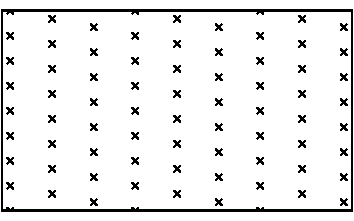
\includegraphics[height=2in]{figs/lec1_lattice}}
\caption{A lattice in $\R^{2}$}
\label{lec1:fig_a_lattice}
\end{figure}

Lattices are a recurring tool in algebra and number theory, for example to prove finiteness of the class group of a number field, or to the efficiently factor rational polynomials. 

More recently, lattices have become a topic of active research in computer science. Algorithmic problems based on lattices (e.g. Shortest and Closest Vector Problems, $\dots$) have found a wide variety of applications; they are used within optimization algorithms, in the design of wireless communication protocols, and perhaps the most active research area, in the development of secure cryptographic primitives (cryptography) and in establishing the insecurity of certain cryptographic schemes (cryptanalysis).  But lattices and their algorithm find applications in various branch of sciences, such as reconstructing molecule composition from mass spectrometry (chemistry), or detecting pulsars (astronomy). 


\section{Notation and Basic Concepts}

We use $\R$ for the real numbers, $\Z$ for the integers and $\N$ for the natural
numbers (positive integers). Correspondingly, we use $\R^n$ and $\Z^n$ to denote
the $n$-dimensional versions for some $n \in \N$. We write generally matrices as
$\mat B$ in uppercase bold, vectors $\vec x \in \R^n$ in lowercase bold and
scalars as $x \in \R$. 

%The Euclidean norm of a vector $\vec x \in \R^n$ is
% denoted $\norm{\vec x} \eqdef (\sum_{i=1}^n x_i^2)^{1/2}$ and the unit Euclidean
% ball in $\R^n$ is denoted by $\ball^n \eqdef \set{\vec x \in \R^n: \norm{\vec x}
% \leq 1}$. For two vectors $\vec x,\vec y \in \R^n$, we denote their inner
% product by $\pr{\vec x}{\vec y} \eqdef \sum_{i=1}^n x_i y_i$.  Given a linear
% subspace $W \subseteq \R^n$, we let $W^\perp = \set{\vec x \in \R^n: \pr{\vec
% x}{\vec y} = 0 \forall \vec y \in W}$ denote the orthogonal complement of $W$.
% We define $\pi_W: \R^n \rightarrow W$ to be the orthogonal projection onto $W$.

For a set $A \subseteq \R^n$, we use $\linsp(A)$ to denote its linear span of
$A$, i.e.~the smallest linear subspace containing $A$. We define the dimension
$\dim(A)$ of $A$ to be the dimension of the linear span, that is, $\dim(A)
:= \dim(\linsp(A))$. 
For two sets $A,B \subseteq \R^n$, $s,t \in \R$, we
define their Minkowski sum $sA + tB := \set{s\vec a + t \vec b: \vec a \in
A, \vec b \in B}$.  

\section{Definitions and Basic Concepts}

The main goal of this lecture is to introduce the basic concept of a lattice,
define one of its basic geometric parameters (the shortest non-zero
vector), and present various equivalent definitions of a lattice. Our abstract 
definition of a lattice is given below:

\begin{definition}[Lattice]
$\lat \subseteq \R^n$ is a lattice if $\lat$ is a discrete additive subgroup of
$\R^n$. $\lat$ is a rank $k$ lattice, or is $k$-dimensional, if $\dim_\R(\lat) = k$.
$\lat$ is said to be full-rank if $\dim_\R(\lat) = n$ (the dimension of the ambient
space).  
\end{definition}

\paragraph{Endowment of $\R^n$.} For what is to come, $\R^n$ will be endowed with {\em some} norm denoted $\|~\cdot~\|$.
A norm induces a metric on $\R^n$ which is non-trivial, and any non-trivial metric on $\R^n$ induces the same topology on $\R^n$. Note that a discrete group must be ``uniformly discrete'', a set $S$ is uniformly discrete in a metric space $X$ if there exists a $\delta > 0$ such that for all $s \in S$, the open ball of radius $\delta$ around $s$ contains no other elements of $S$ than $s$ itself.

Another endowment that we will use is its unique Lesbegue measure, denoted $\vol(\cdot)$; for a {\em measurable} set $S \subset \R^n$, the volume $\vol(S)$ is a non-negative real number or $\infty$. We recall that a measure is sub-additive under union and additive under disjoint union: 

\begin{enumerate}
	\item $\vol\left(\bigcup_i S_i \right) \leq \sum_i \vol\left(S_i \right)$
	\item $\vol\left(\bigsqcup_i S_i \right) = \sum_i \vol\left(S_i \right)$
\end{enumerate}

Being a Lesbegue measure on $\R^n$, it is also invariant by translation, is homogeneous, and is normalized on the canonical hypercube: 
\begin{enumerate}
	\item $\forall \vec x \in \R^n, \vol(S + \vec x) = \vol(S)$ 
	\item $\forall \vec T \in \R^{n \times n}, \vol(\vec T \cdot S) = |\det(\vec T)| \cdot \vol(S)$ 
	\item $\vol([0, 1]^n) = 1$ 
\end{enumerate}
The second property implies invariance under rotations $\vec T \in \mathcal O_n(\R)$. One can easily deduce that a bounded measurable set has finite measure, and that a set with non-empty interior has strictly positive measure.

Issues of measurability shall not arise in this course and will be ignored; most bodies $S \subset R^n$ we will encounter are convex or are a finite combination of convex bodies. 

\begin{remark} The term lattice is quite overloaded in the literature, and can also refer to an order, or to subgroup of other groups than $\R^n$. The lattices as defined above are sometimes referred to as ``point lattices''. The term ``Euclidean lattices'' is also used when the considered metric is Euclidean.
\end{remark}

\begin{proposition}\label{prop:minimumExists} A non-trivial subgroup $L \subset \R^n$ is discrete if and only if it admits a strictly positive minimal distance, that is if $\min_{\vec x \neq \vec y \in L} \|\vec x - \vec y\|$ is well defined and strictly positive.
\end{proposition}
Because a lattice $L$ is a group, its minimum distance can be rewritten as $\min_{\vec x \in L \butzero} \|\vec x\|$. It will be denoted $\lambda_1(L)$.

\begin{proof}
Having a minimal distance immediately implies discreteness: around each element of the subgroup $L$, we can take the open ball of radius $\lambda_1/2$, which does not include any other point in $L$.

For the other direction, we will show that the minimal distance is attained and is strictly positive.
By discreteness and non-triviality of $L$, the greatest lower bound \[\lambda_1~=~\inf~\{ \|\vec x\| : \vec x \in L \butzero \}\] exists and is strictly positive.
Consider the open ball $B$ of radius $2\lambda$ about the point $0$.
By definition of $\lambda$, the ball $B$ will include at least one non-zero element $\vec x \in L$.
This ball is bounded and thus has finite volume $V := \vol(B)$.
Moreover, an open ball $C$ of radius $\lambda/2$ has a strictly positive volume.
For any two $\vec x , \vec y \in L \cap B$, the intersection $\vec x + C \cap \vec y + C$ is empty, by definition of $\lambda$.
Thus the union
\[
U = \bigsqcup_{\vec x \in B \cap L}  \vec x + C
\]
is disjoint, and therefore has volume
\[
\vol(U) = \sum_{\vec x \in B \cap L} \vol (\vec x + C) = \sum_{\vec x \in B \cap L} \vol (C) = |B\cap L| \vol(C).
\]
Note that $U$ is also bounded (it is a subset of the open ball $D$ of radius $5\lambda / 2$) and therefore has finite volume. Therefore, $|B \cap L|$ is finite. This finite set has an element with minimal norm, which by construction is $\lambda$. Thus the infimum is attained and is thus a minimum.
\end{proof}
\begin{exercise}Provide two counterexamples when the either assumption of the above proposition is not met:
\begin{itemize}
	\item A finitely generated subgroup of $\R$ that is not discrete, and doesn't admit a minimal distance
	\item A discrete subset (but not uniformly) of $\R$ that is not a group, and doesn't admit a minimal distance
\end{itemize}
\end{exercise}

\subsection{Bases}

\begin{definition}[Basis of a lattice] A matrix $\vec B = [\vec b_1 \dots \vec b_k] \in \R^{n \times k}$ is a basis of a lattice $L \subset \R^n$ if its column vectors are linearly independent over $\R$ and the $\Z$-span of its columns is exactly $L$, i.e.
\[\lat(\vec B) := \vec B \cdot \Z^k = L.\]
\end{definition}
The goal of this section is to prove that all lattices admit a basis. By definition, one can find a set of linearly independent vectors in $L$. We will show that such a set generates a sublattice of $L$ of finite index. From there, we will reconstruct a basis. For the first step, we resort to the \emph{fundamental parallelepiped}: if $\vec B \in \R^{m \times k}$ has linearly independent columns we denote $\para(\vec B):= \vec B \cdot [-1/2, 1/2)^n$ the parallelepiped spanned by $\vec B$.

\begin{proposition}\label{prop:fundamentalDomain} For any basis $\vec B$ of $L$, $\para(\vec B)$ is a fundamental domain of $L$, that is any $\vec t \in \Span_\R(L)$ can be uniquely written as $\vec t = \vec x + \vec e$ where $\vec x \in L$ and $\vec e \in \para(\vec B)$.
\end{proposition}
\begin{proof}
If $L = \{ 0 \}$, then $\vec t = 0$, so we take $\vec x = 0$ and $\vec e = 0$ and we are done.
Otherwise, let $\vec t \in \Span_\R(L)$.
As an element of the $\R$-span, $\vec t$ can be written as a linear combination
\[
\vec t = c_1 \vec b_1 + \ldots + c_k \vec b_k,
\]
where $k >0$ is the dimension of the lattice and each $c_i \in \R$.
Now define the rounding function $\lfloor \cdot \rceil : \R \rightarrow \Z$ that rounds a real number $x$ to the largest integer not greater than $x + 0.5$ (that is, the familiar rounding function where half-integers are rounded up to the next integer).
Consider now $\vec x := \lfloor c_1 \rceil \vec b_1 + \ldots + \lfloor c_k \rceil \vec b_k$.
This is a $\Z$-linear combination of the basis vectors in $\vec B$, so $\vec x \in L$.
Define \[\vec e := \vec t - \vec x = (c_1 - \lfloor c_1 \rceil ) \vec b_1 + \ldots + (c_k - \lfloor c_k \rceil)  \vec b_k.\]
Each $c_i - \lfloor c_i \rceil \in [- 1/2 , 1/2)$, so $\vec e \in \para(\vec B)$.

It remains to show uniqueness.
Suppose we have two different such representations $\vec t = \vec x + \vec e = \vec x' + \vec e'$, where $\vec x \neq \vec x'$ and $\vec e \neq \vec e'$.
Then $0 = \vec x - \vec x' + \vec e - \vec e'$.
Since $\vec x - \vec x' \in L$, we also require that $\vec e - \vec e' \in L$.
But $\vec e, \vec e' \in \para(\vec B)$, so $\vec e - \vec e' \in \vec B \cdot (-1, 1)^k \cap L = \{ 0 \}$.
Thus $\vec e = \vec e'$ and $\vec x = \vec x'$ follows.
\end{proof}

\begin{proposition}\label{lem:FiniteQuotient} Let $L'$ be a lattice admitting a basis $\vec B$, and $L$ a superlattice of $L'$ of the same dimension. The index of the quotient group $|L / L'| < \infty$ is finite.
\end{proposition}
\begin{proof}
Given $L' \subseteq L$ have the same rank, we know their $\R$-spans are the same.
Thus for every coset in $L/L'$, we can lift to an element in $\vec s \in L \subseteq \Span_\R(L)$.
Let $S$ be a set consisting of a lifted element for every coset in $L / L'$.
Then $|S| = |L / L'|$.
Now, by Proposition \ref{prop:fundamentalDomain} $\vec s = \vec t_s + \vec e_s$ for some $\vec t_s \in L'$ and $\vec e_s \in \para (\vec B)$.
Let $E$ be the set of all $\vec e$ resulting from this decomposition.
Since no two lifts $\vec s$ differ by an element of $L'$, we know that each $\vec e$ is unique to each $\vec s \in S$, and so $|S| = |E|$.
Furthermore, $E$ is discrete since $L$ is discrete.
Following the same argument as in the proof of Proposition \ref{prop:minimumExists}, we know that only finitely many elements of the uniformly discrete set $E$ can be contained in the bounded set $\para (\vec B)$.
But since $E \subseteq \para (\vec B)$, $E$ is finite, and therefore so is $|L/L'|$.
\end{proof}

% \shane{One can mention here that the above proposition has an algebraic version:
% The lattice $L$ is a finitely generated abelian group with rank $r$.
% Its quotient by a subgroup $L'$ of rank $r$ is finite.}

% \begin{lemma} Let $\lat \subset \R^n$ be a lattice and $\vec b_1, \dots, \vec b_k \in \lat$ be arbitrary lattice vectors. Let us then define $W := span(\vec b_1, \dots, \vec b_k)^{\perp}$. The projection $\pi_{W}$ onto $W$ is a lattice.
% \end{lemma}

% \begin{proof}
% \simona{I don't have any better proof than proof for Lemma 8 in the old lecture notes, so I would go for the same one.}
% \end{proof}

% \begin{lemma}  Let $\lat \subset \R^n$ be a $k$-dimensional lattice.
% \simona{Shane and I discussed it but we didn't find the way to go around the definition of primitive (and rely, for example, on the fundamental domain, so I guess we would again just copy the proof of Lemma 8 of the old lecture notes}.
% \end{lemma}

\begin{theorem}\label{thm:alwaysABasis} Any lattice admits a basis.
\end{theorem}
\begin{proof}
Let $L \subset \R^n$ be a lattice of rank $k$. Let $\vec B \subset \R^{n \times k}$ be matrix whose column vectors are linearly independent vectors of $L$. By Proposition~\ref{lem:FiniteQuotient}, the quotient $G = L/\lat(\vec B)$ is finite. 

If the quotient is trivial then $L=\lat(\vec B)$, and $\vec B$ is a basis of $L$, we are done.
Otherwise, choose some $\vec x \in L \setminus \lat(\vec B)$ of prime order $p$ in G.
Because $p \vec x \in \lat(\vec B)$, it can be written as $\vec x = \vec B \vec y$ where $\vec y \in \frac 1 p \Z^k$.
Without loss of generality (by permutation of the basis vectors of $\vec B$), we can assume that its first coordinate is not integral: $\vec y = (\frac a p, \vec y')$ where $a \neq 0 \bmod p$.
We can further assume that $a=1$, by replacing $\vec x$ by $c \vec x - \frac {ac - 1} p \vec b_1$ where $ac = 1 \bmod p$.

The claim is that $\vec B' := (\vec x, \vec b_2, \dots, \vec b_n)$ generates a sublattice of $L$ that is a strict superlattice of $\lat(\vec B)$, namely $\lat(\vec B) + \vec x \Z$.
That it is a sublattice of $L$ is trivial: by construction $\vec x \in L$ and for all $i$, $\vec b_i \in L$.
To show that it is a superlattice of $\lat(\vec B)$, it suffices to prove that $\vec b_1 \in \lat(\vec B')$.
Recall that $\vec x = \vec B \cdot (\frac 1 p, \vec y')$ for some $\vec y'$ in $\frac 1 p \cdot \Z^{k-1}$.
Simply note that $\vec b_1 = p \vec x - \vec B' \cdot (0, p \vec y')$.
Finally, because $\vec x \not \in \lat(\vec B)$, the inclusion $\lat(\vec B) \subset \lat(\vec B')$ is indeed strict.

We conclude by repeating the above process, replacing $\vec B$ by the newly constructed $\vec B'$, until $\vec B$ is indeed a basis of $L$.
Note that since $\lat(\vec B) \subsetneq \lat(\vec B')$, the size of the quotient group $|L / \lat(\vec B)|$ is finite and stricly decreases at each step.
Therefore it must terminate after some finite number of steps, at which point $|L/\lat(\vec B)| = 1$, and $\lat(\vec B) = L$.
\end{proof}

% \begin{proof} (by induction)
% Let us take $\vec x \in \lat \setminus \{0\}$ and let $\lat_1 = \Span(\vec y) \cup \lat$. As $\lat_1$ is a one-dimensional sub-lattice of $\lat$, by Proposition 3, we know there exist a shortest non-zero vector of $\lat_1$. Let us denote it by $\vec b_1$. Now we need to show that $\vec b_1$ is a basis of $\lat_1$, namely, we want to show that $\lat_1 = \lat(\vec b_1)$. We know $\lat(\vec b_1) \subseteq \lat$, so we want to show that $\lat \subseteq \lat(\vec b_1)$.

% By proposition 5, we know that for any $\vec x \in \lat$, $\exists \vec v \in \lat(\vec b_1), \vec e \in \para(\vec B)$ such that $\vec x = \vec v + \vec e$. If $\vec e$ is a all zero vector, then $\vec x$ is also in $\lat(\vec b_1)$, so $\lat \subseteq \lat(\vec b_1)$. If not, we then have $\vec e = \vec x - \vec v \in \lat$ which is then strictly shorter than $\vec b_1$ and that leads to contradiction with the initial assumption that $\vec b_1$ is the shortest vector.

% Let us now observe $k \geq 2$, and let us take $\lat_2 = \pi_{\vec b_1^{\perp}}(\lat)$. By Lemma 7, $\lat_2$ is a lattice, and its dimension is $k-1$. By inductive hypothesis, $\lat_2$ admits a basis, so we can take $\vec b_2', \dots, \vec b_k'$ to be its basis. Moreover, we can find  $\vec b_2, \dots, \vec b_k \in \lat$ such that $\pi_{\vec b_1^{\perp}}(\vec b_j) = \vec b_j'$ for each $j \in \{2, \dots, k\}$. By Lemma 8, $\vec b_1, \dots, \vec b_k$ is a basis of a $k$-dimensional lattice $\lat$.
% \end{proof}

\begin{proposition}\label{prop:basesOfLattice} For any two bases $\vec B, \vec B' \in \R^{n \times k}$ of the same lattice $L$ of rank $k$, there exists $\vec U \in \GL_k(\Z)$ such that $\vec B' = \vec B\vec U$. Conversely, if $\vec B$ is a basis of $L$, so is $\vec B \vec U$ for any unimodular matrix $\vec U \in \GL_k(\Z)$.
\end{proposition}

\begin{proof}
The lattices $\lat (\vec B), \lat(\vec B')$ are equal and therefore sublattices of one another.
Since $\lat (\vec B) \subseteq \lat(\vec B')$, each basis vector in $\vec B'$ is an integer linear combination of basis vectors in $\vec B$.
This can be written as $\vec B' = \vec B \vec M$ for some $\vec M \in \Z ^{k \times k}$.
The matrix $M$ has non-zero determinant, since both $\vec B$ and $\vec B'$ have rank $k$.
The same is true for the other direction of the inclusion, i.e. $\vec B = \vec B' \vec M'$ for some $\vec M' \in \Z^{k \times k}$ with rank $k$.
Combining these two facts tells us
\[
\vec B = \vec B \vec M \vec M'.
\]
The matrix $\vec B$ is non-singular, so the above holds if and only if $\vec M \vec M' = \vec I_k$.
Since both of $\vec M$ and $\vec M'$ are integer valued, their determinants are also integers, and thus $\vec M, \vec M' \in \GL_n(\Z)$.

For the converse, we argue as above that for any basis $\vec B$, the lattice generated by $\vec B \vec U$ for any $\vec U \in \Z^{k \times k}$ is a sublattice of $\lat(\vec B)$, and so $\lat(\vec B \vec U) \subseteq \lat (\vec B)$.
Now if $\vec U$ is unimodular, then $\vec U^{-1} \in \Z^{k \times k}$ and so by the same argument, $\lat (\vec B ) = \lat(\vec B \vec U \vec U^{-1}) \subseteq \lat (\vec B \vec U)$.
Therefore $\lat (\vec B ) = \lat (\vec B \vec U)$.
\end{proof}

\subsection{Covering, Packing, Tiling}
Subsets of $\R^n$ are called coverings, packings or tilings based on how well they "fill up" the space between lattice points.
A set $S$ is covering if the repeated pattern of $S$ at every lattice point will cover all of $\Span_\R(L)$.
Similarly, a set $S$ is packing if no repeated instance of $S$ will intersect with another instance of $S$.
Tiling is when both of these are true: every point of $\Span_\R(L) $ can be found in exactly one instance of $S$, when $S$ is repeated at every lattice point.
Formally,
\begin{definition}[Covering, Packing, Tiling]
Let $S \subseteq \Span_\R(L)$.
\begin{enumerate}
\item The set $S$ is said to be $L$-covering if $L + S = \Span_\R(L)$.
\item $S$ is $L$-packing if for any pair $\vec t, \vec u \in L$, $\vec t + S \cap \vec u +S = \emptyset$.
\item $S$ is $L$-tiling if it is both packing and covering.
\end{enumerate}
\end{definition}
All these properties can be though as in term of the union underlying the notation $L + S:= \bigcup_{\vec x \in L} S + \vec x$: covering means this union is the whole space, and packing means this union is disjoint. Tiling is a synonym of being a fundamental domain for $L$.

The fundamental parallelepiped $\para(\vec B)$ is a tiling with respect to $L$, as a corollary of Proposition \ref{prop:fundamentalDomain}.
Since the concept of covering, packing and tiling are so closely linked, we often use an abbreviation of notation that hopefully doesn't lead to any confusion.

\begin{proposition}\label{prop:pack_cov_volume_vound}
Let $L \subseteq \R^n$ be a $k$-dimensional lattice and let $S \subseteq \Span_\R(L)$ be a measurable set.
If $S$ is $L$-(covering, packing, tiling), then $\vol(S) \quad ( \geq,\leq,=) \quad \vol(\para(\vec B))$.
In particular, every tiling has the same volume.
\end{proposition}

\begin{proof} The proof proceeds with a collage.
Let us simplify the notation $P = \para(\vec B)$.
Cut $S$ into the disjoint union $S = \bigsqcup_{\vec x \in L} S \cap (P + \vec x)$.
Move each piece back to $P$ by translating it by $-\vec x$, and glue them back as $T := \bigcup_{\vec x \in L} \left((S - \vec x) \cap P\right)$.
In particular $T \subseteq P$.
By the properties of the Lebesgue measure, $\vol(T) \leq \vol(P)$ and $\vol(T) \leq \vol(S)$. 

If $S$ is packing, then the union defining $T = \bigcup_{\vec x \in L} \left((S - \vec x) \cap P\right)$ is disjoint because the $(S - \vec x)$ are disjoint.
So $\vol(T) = \sum_{\vec x} \vol((S - \vec x) \cap P) = \sum_{\vec x} \vol(S \cap (P + \vec x)) = \vol(S)$ and we conclude that $\vol(S) \leq \vol(P)$. 

If $S$ is now covering, we claim that $T = P$, and we conclude that $\vol(S) \geq \vol(P)$. Indeed, $T = \bigcup_{\vec x \in L} \left((S - \vec x) \cap P\right) = \left(\bigcup_{\vec x \in L} (S - \vec x)\right) \cap P = \Span_\R(L) \cap P = P$.
\end{proof}

\subsection{Determinant, Volume and Density}
The above leads us to define the determinant of a lattice (sometimes called the volume, or less frequently but more accurately the co-volume).

\begin{definition} The determinant $\det(L)$ is defined as $\sqrt{|\det(\vec B^t \vec B)|}$ for any basis $\vec B$ of L.
\end{definition}
It follows from Proposition \ref{prop:basesOfLattice} that this value does not depend on the choice of basis.
In that sense it is an \emph{invariant} of the lattice.
Note that if $L$ is full rank, then its determinant can be computed more simply as $|\det (\vec B)|$.
The determinant can be thought as the inverse of the density of the lattice: tiling the space as $\bigcup_{\vec x \in L} \para(\vec B) + \vec x$, each tile has volume  $\vol(\para(\vec B)) = \det(L)$, and contains one lattice point. 

This density intuition can be formalized as the following statement, (which applies to any choice of norm).
\begin{theorem}\label{thm:densityTheorem} Let $L \subset \R^n$ be a full-rank lattice, and let $\mathcal B$ denote the closed ball of radius $1$, $\mathcal B := \{ \vec x \in \R^n \mid \|\vec x\|\leq 1\}$. Then, 
\[ \lim_{r \rightarrow \infty} \frac {\left |r\mathcal B \cap L\right |} {r^n\vol(\mathcal B)} = \frac 1 {\det ( L)}.\]
\end{theorem}

We will prove Theorem \ref{thm:densityTheorem} using a packing and covering argument. 
%, for which we need the concept of the \emph{covering radius}. 
%\leo{Todo: tweak the lemma to use the radius of any given fundamental domain rather than the covering radius. This allows to delay def of cov radius and voronoi cell to a latter class.}

% \begin{definition}
% For a lattice $L \in \R^n$, the \emph{covering radius} $\mu(L)$ is the following non-negative real number
% \[
% \mu(L) := \sup_{x \in \Span(L)} \{ \min_{\vec y \in L } \{ \| \vec x - \vec y \| \}.
% \]
% When the lattice in question is clear from the context, we write only $\mu$.
% \end{definition}
% Note above that, inside the $\sup$, we take the \emph{minimum} over all lattice points, not the infimum.
% The proof that such a minimum exists is essentially the same as that for Proposition \ref{prop:minimumExists}, so we omit it.
% From the existence of the first minimum, we can infer that $\mu \geq \lambda_1 /2> 0$.

% We may also show that the covering radius is finite.
% By Theorem \ref{thm:alwaysABasis}, every lattice has a basis.
% Then by Proposition \ref{prop:fundamentalDomain}, every point $\vec x \in \Span_\R(L)$ can be decomposed uniquely into $\vec x = \vec t + \vec e$, where $\vec t \in L$, and $\vec e \in \para(\vec B)$.
% Thus for any such point $\vec x$, the distance $\min_{\vec y \in L } \{ \| \vec x - \vec y \|\} \leq \| \vec x - \vec t \| \leq \| \vec e\|$.
% By the triangle inequality for norms, $\|\vec e  \| \leq \sum_{i = 1}^k \vec \| \vec b_i\|$, which is indeed finite.

\begin{proposition}\label{prop:packingArgument} Let $T$ be a bounded tiling for a lattice $L$, and $\mu = \sup_{\vec x \in T} \|x\|$. Then, for any radius $r > \mu$ it holds that $\frac{ (r-\mu)^n}{\det(L)} \leq \frac {|L \cap r\mathcal B|} {\vol(\mathcal B)} \leq \frac{ (r+\mu)^n}{\det(L)}$.
\end{proposition}
\begin{proof} %\leo{Maybe with nice drawings !}\\
We first show the right-hand bound.
Let $T$ be a tiling set of $L$ that is contained in $\mu\mathcal{B}$.
This is a covering set by definition, so $\R^n = L + T$.
Furthermore, $(L \cap r\mathcal{B})+ T \subseteq (r+\mu)\mathcal{B}$ by the triangle inequality.
This gives \[\vol((L \cap r\mathcal{B})+ T) \leq \vol( (r+\mu)\mathcal{B}) = (r + \mu)^n \vol (\mathcal{B}).\]
But since $T$ is tiling, and any tiling set has volume $\det(L)$, the left hand side can be written as $\sum_{\vec x \in L \cap r\mathcal{B} } \vol (T) = |L \cap r\mathcal{B}| \det(L)$.
Thus $|L \cap r\mathcal{B}| \det(L) \leq  (r + \mu)^n \vol (\mathcal{B})$ and the right hand side follows.

For the left-hand bound, note first that $(r - \mu)\mathcal{B} \subseteq (L \cap r\mathcal{B})+ T$.
Then, for the same reasoning as before, we see
\[
(r-\mu)^n\vol(\mathcal{B}) \leq |L \cap r\mathcal{B}| \det(L),
\]
and the bound follows.
\end{proof}

\begin{proofof}{Theorem~\ref{thm:densityTheorem}}
This is an immediate corollary of Proposition \ref{prop:packingArgument}, by choosing $T = \para(\vec B)$ for any basis $\vec B$ of $L$, noting that $\mu \leq \frac 1 2 \sum \|\vec b_i\|$ is finite. 
Divide across by $r^n$ and take the limit.
\end{proofof}

\section{Minkowski's First Theorem}

With all the above prequisite, there is not much left to do to reach Minkowski's first theorem and Minkowski's bound. It is often demonstrated via the so-called Blichfeldt lemma, which at this point is merely the contrapositive of the volume bound for packing (Proposition~\ref{prop:pack_cov_volume_vound}).

\begin{lemma}[Blichfeldt] For any lattice $L$ and any measurable set $S \subset \Span_\R(L)$ such that $\vol(S) > \det(L)$, there exist distinct $\vec x, \vec y \in S$ such that $\vec x - \vec y \in L$.
\end{lemma}

\begin{theorem}[Minkowski Convex Body Theorem]  For any lattice $L$ of rank $n$ and any symmetric ($S = -S$) {\em convex} set $S \subset \Span_\R(L)$ such that $\vol(S) > 2^n \cdot \det(L)$, there exists a non-zero lattice vector in $S$: $|S \cap L| > 1$.
\end{theorem}
\begin{proof} Apply Blichfeldt lemma to the lattice $L' = 2 L$, of determinant $\det(L') = 2^n \cdot \det(L)$, and obtain distinct $\vec x, \vec y \in S$ such that $\vec x - \vec y \in L'$. Note that $\vec z := \frac {\vec x - \vec y} 2 \in L$, and because $S$ is symmetric and convex, $\vec z$ also belongs to $S$. Note finally that $\vec z$ is non-zero since $\vec x$ and $\vec y$ are distinct.
\end{proof}

\begin{theorem}[Minkowski Bound] The minimal distance of any full rank lattice $L \subset \R^n$ is bounded by below: $\lambda_1(L) \leq	2 \cdot (\frac {\det(L)} {\vol(\mathfrak B)})^{\frac 1 n}$, where $\mathfrak B$ is the ball of radius $1$: $\mathfrak B = \left\{\vec x \in \R^n \mid \|\vec x\| \leq 1 \right\}$.
\end{theorem}

In particular, for the Euclidean norm $\|\vec x\| := \sqrt{\sum x_i^2}$ (a.k.a. the $\ell_2$ norm) the unit ball $\mathfrak B$ has volume $\vol(\mathfrak B) = \frac {\pi^{n/2}} {\Gamma(\frac n 2 + 1)}$ where $\Gamma(x+1) \sim \sqrt{2 \pi x} (x/e)^x$ (Stirling's approximation).
Hence, $n$-dimensional lattice of rank $n$ have a normalized minimal distance of at most:
\[ \frac {\lambda_1^{(2)} (L)} {\det(L)^{1/n}} \leq \sqrt{\frac {2n} {\pi e}} + o(\sqrt n). \]
Note that because the restriction of an $\ell_2$-ball to any subspace of $\R^n$ is still an $\ell_2$-ball, this bound is not limited to full-rank lattices. 

\end{document}
